\documentclass[tikz,border=5mm]{standalone}
\begin{document}
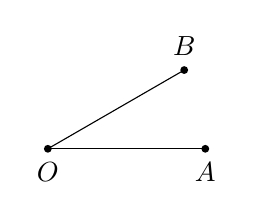
\begin{tikzpicture}
    % 画线段
    \draw (0,0) -- (2,0);
    
    % 旋转线段
    \draw (0,0) -- (30:2);
    
    % 标注点
    \node [circle,fill=black,inner sep=1pt,label=below:$O$] at (0,0) {};
    \node [circle,fill=black,inner sep=1pt,label=below:$A$] at (2,0) {};
    \node [circle,fill=black,inner sep=1pt,label=above:$B$] at (30:2) {};
\end{tikzpicture}
\end{document}